\documentclass{ximera}

\author{Anna Davis} \title{MTH 160 Homework 1} 

\begin{document}

\begin{abstract}

\end{abstract}
\maketitle
 \textit{Certificate due: 8/26/2020 at 11:59 p.m.}
\begin{problem}\label{prob:160hom1prob1}
The collection of all inputs into a function is called the
\begin{multipleChoice}  
\choice{Range}  
\choice{Input Set}  
\choice[correct]{Domain}  
\choice{Image}  
\end{multipleChoice}  
\end{problem}

\begin{problem}\label{prob:160hom1prob2}
The collection of all outputs of a function is called the
\begin{multipleChoice}  
\choice[correct]{Range}  
\choice{Output Set}  
\choice{Domain}  
\choice{Pre-image}  
\end{multipleChoice}  
\end{problem}

\begin{problem}\label{prob:160hom1prob3}
Label each relation using a drop-down menu.
\begin{enumerate}
    \item The relation represented by the diagram below is \wordChoice{\choice[correct]{a function}, \choice{not a function}}
    \begin{image}
   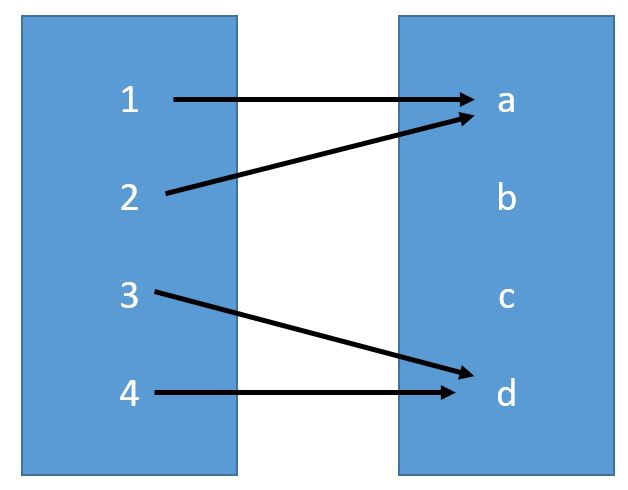
\includegraphics[height=1in]{160H1Function1.JPG}
 \end{image}
 \item The relation represented by the diagram below is \wordChoice{\choice{a function}, \choice[correct]{not a function}}
    \begin{image}
   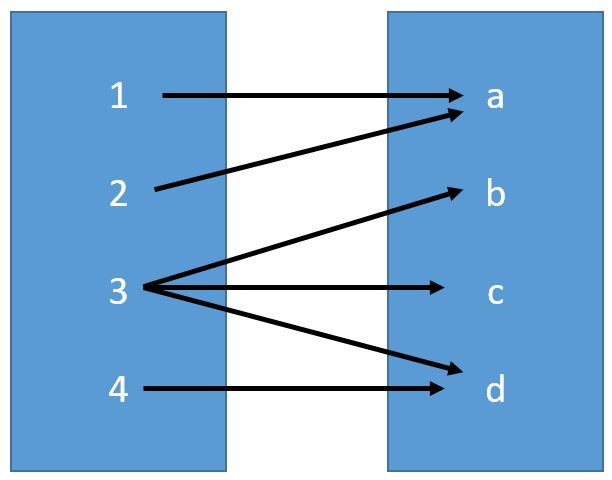
\includegraphics[height=1in]{160H1Function2.JPG}
 \end{image}
 \item The graph below represents a relationship between $x$ and $y$. \wordChoice{\choice{$y$ is a function of $x$}, \choice[correct]{$y$ is not a function of $x$}}
    \begin{image}
   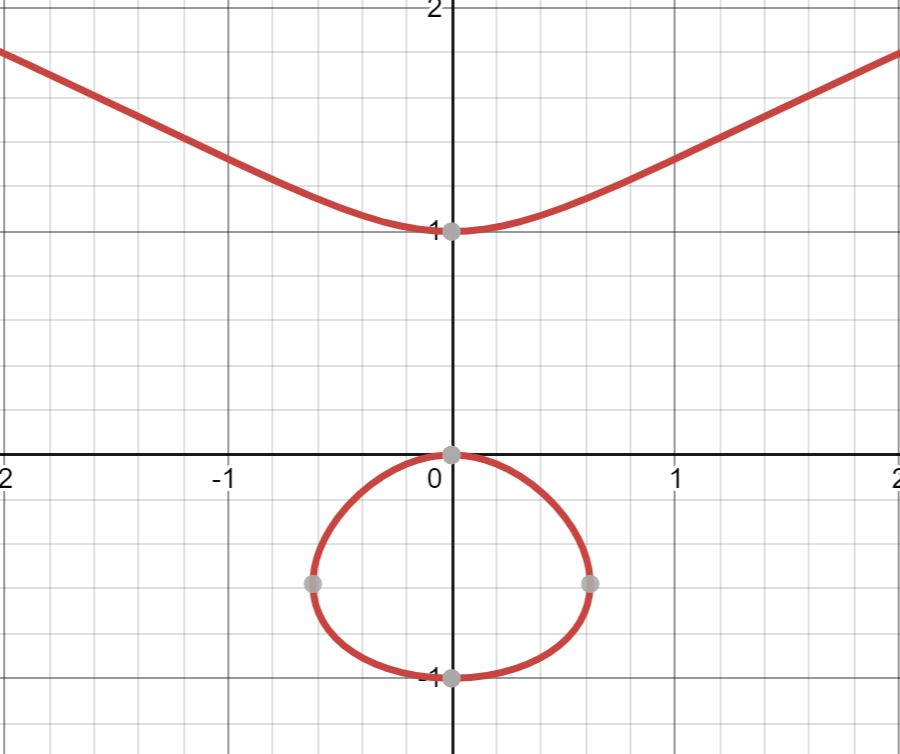
\includegraphics[height=1in]{160H1Function3.JPG}
 \end{image}
 \item The graph below represents a relationship between $x$ and $y$. \wordChoice{\choice[correct]{$y$ is a function of $x$}, \choice{$y$ is not a function of $x$}}
    \begin{image}
   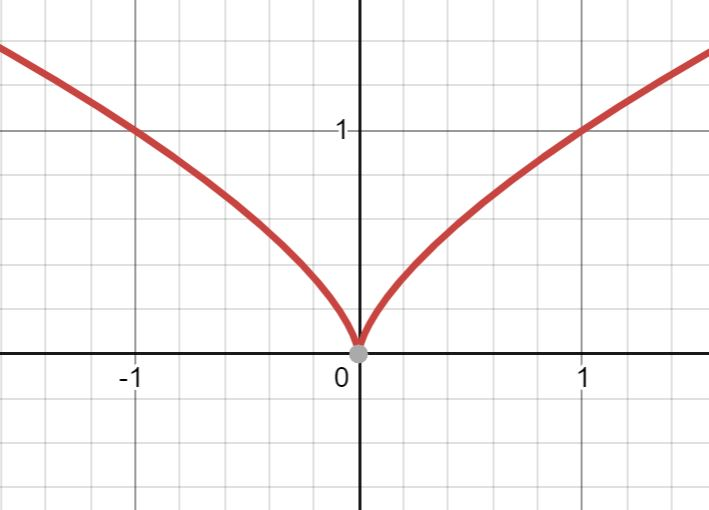
\includegraphics[height=1in]{160H1Function4.JPG}
 \end{image}
  \item The graph below represents a relationship between $x$ and $y$. \wordChoice{\choice[correct]{$x$ is a function of $y$}, \choice{$x$ is not a function of $y$}}
  (Hint: read the wording of the choices carefully!)
    \begin{image}
   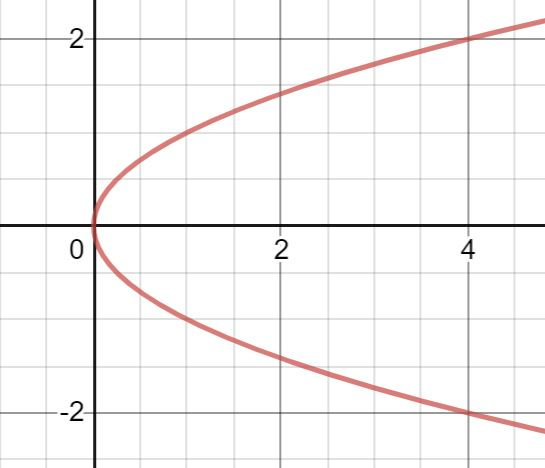
\includegraphics[height=1in]{160H1Function5.JPG}
 \end{image}
\end{enumerate}
\end{problem}

\begin{problem}\label{prob:160hom1prob4}
The graph of function $f$ appears below.  Use the graph to evaluate the function.
\begin{image}
   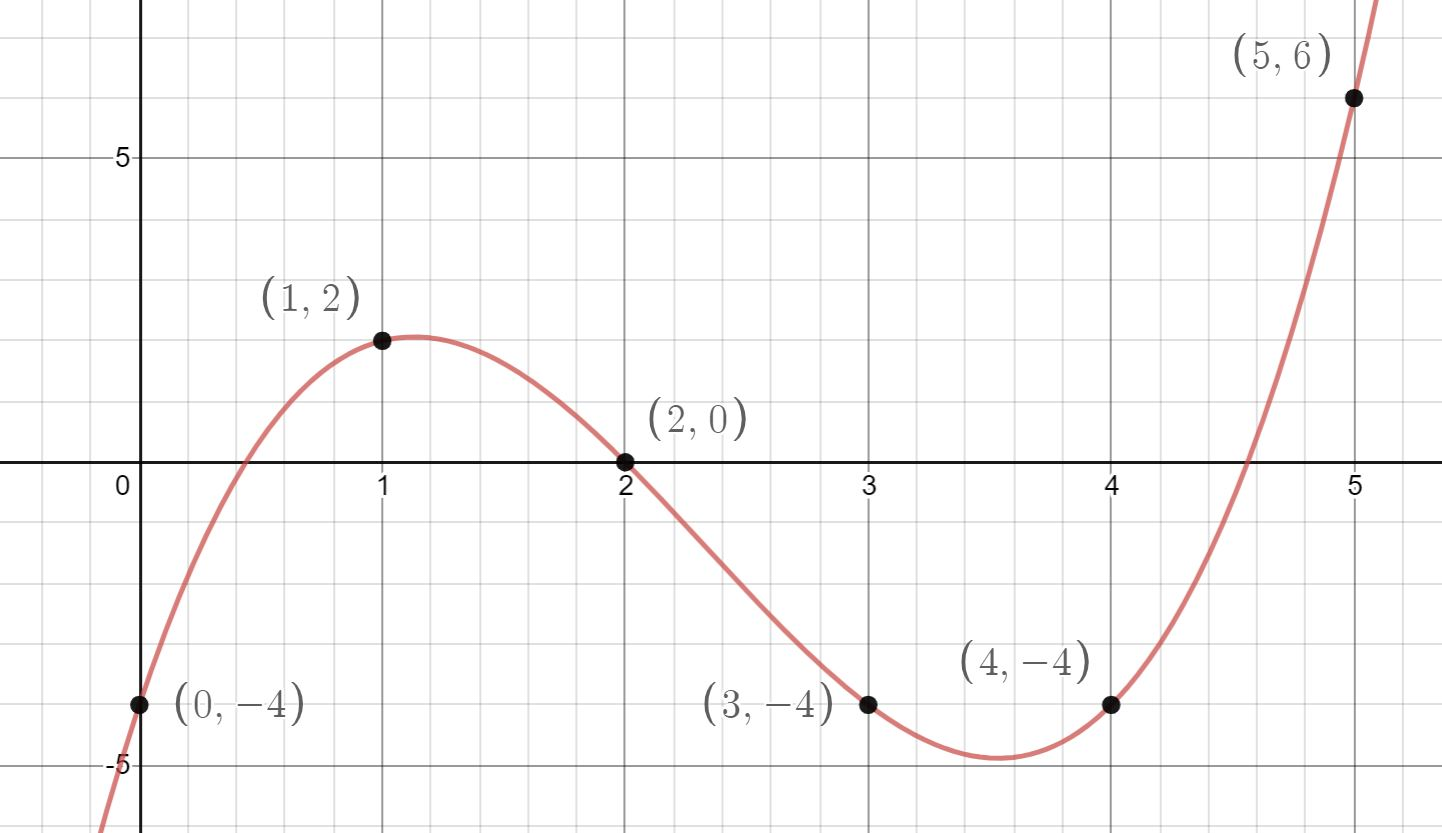
\includegraphics[height=1in]{160H1Function6.JPG}
 \end{image}
 $$f(0)=\answer{-4},\quad f(5)=\answer{6},\quad f(3)=\answer{-4}$$ $$f(2)=\answer{0},\quad f(1)=\answer{2},\quad f(4)=\answer{-4}$$
\end{problem}

\begin{problem}\label{prob:160hom1prob5}
Evaluate the function, as indicated.
\begin{enumerate}
    \item $f(x)=x^3-x+1$ $$f(0)=\answer{1},\quad f(2)=\answer{7},\quad f(-2)=\answer{-5}$$
    \item $f(x)=-x^2+4x-8$ $$f(0)=\answer{-8},\quad f(2)=\answer{-4},\quad f(-1)=\answer{-13}$$
    \item $f(x)=\frac{1}{x}+x$ $$f(1)=\answer{2},\quad f(2)=\answer{2.5},\quad f(-1)=\answer{-2}$$
    \item $f(x)=\frac{1}{x}$  $$f\left(\frac{5}{9}\right)=\frac{\answer{9}}{\answer{5}}$$
    Enter your answer as a fraction.
    \item $f(x)=2^x$ $$f(5)=\answer{32},\quad f(0)=\answer{1},\quad f(-1)=\frac{\answer{1}}{\answer{2}}$$
\end{enumerate}
\end{problem}

\begin{problem}\label{prob:160hom1prob9}
Expand.
$$(a+b)^2=a^2+\answer{2}ab+\answer{b^2}$$
\begin{hint}
$(a+b)^2=(a+b)(a+b)$
\end{hint}
$$(a-5)^2=a^2-\answer{10}a
+\answer{25}$$
\end{problem}

\begin{problem}\label{prob:160hom1prob6}
Let $f(x)=2x^2-3x+4$ evaluate each expression.

$$f(a)=\answer{2a^2-3a+4}$$

$$f(h+2)=\answer{2}h^2+\answer{5}h+\answer{6}$$
\end{problem}

\begin{problem}\label{prob:160hom1prob7}
Let $f(x)=-x^2+2x-7$ evaluate each expression.

$$f(a-2)=\answer{-1}a^2+\answer{6}a-\answer{15}$$

$$f(3b)=\answer{-9}b^2+\answer{6}b-7$$
\end{problem}

\begin{problem}\label{prob:160hom1prob8}
Given a graphical representation of a relationship between $x$ and $y$, we can determine whether $y$ is a function of $x$ by using the $\answer[format=string]{vertical}$ line test.
\end{problem}
\end{document} 